\documentclass[10pt]{article}
\usepackage[a4paper,margin=14mm]{geometry}
\usepackage{amsmath,amssymb,mathtools}
\usepackage{xcolor,tikz,fancyvrb,fontspec,multicol,booktabs,array}
\usetikzlibrary{arrows.meta,positioning,fit,calc,backgrounds,decorations.pathreplacing}
\pagestyle{empty}
\setlength{\parindent}{0pt}
\setlength{\parskip}{4pt}
\setlength{\columnsep}{8mm}

\definecolor{navy}{RGB}{35,51,83}
\definecolor{blue}{RGB}{50,105,160}
\definecolor{teal}{RGB}{24,132,125}
\definecolor{green}{RGB}{42,125,73}
\definecolor{orange}{RGB}{210,120,38}
\definecolor{red}{RGB}{170,60,52}
\definecolor{paper}{RGB}{248,249,252}
\definecolor{muted}{RGB}{102,110,125}
\newfontfamily\leanfont{DejaVu Sans Mono}
\newenvironment{lean}{\Verbatim[fontsize=\small,frame=single,framesep=1.8mm,rulecolor=\color{blue!45},formatcom=\leanfont]}{\endVerbatim}
\newenvironment{leansmall}{\Verbatim[fontsize=\scriptsize,frame=single,framesep=1.5mm,rulecolor=\color{blue!35},formatcom=\leanfont]}{\endVerbatim}
\newcommand{\code}[1]{{\leanfont #1}}
\newcommand{\yes}{\textcolor{green}{\bfseries YES}}
\newcommand{\no}{\textcolor{red}{\bfseries NO}}
\newcommand{\decision}[1]{\textcolor{navy}{\bfseries #1}}
\tikzset{
  box/.style={draw=navy!55, rounded corners=2mm, fill=paper, align=center, inner sep=3mm},
  theorem/.style={box, fill=blue!8, draw=blue!65},
  normal/.style={box, fill=green!9, draw=green!65},
  caution/.style={box, fill=orange!10, draw=orange!70},
  bad/.style={box, fill=red!8, draw=red!65},
  flow/.style={-{Latex[length=2.5mm]}, thick, draw=navy!75},
  label/.style={font=\scriptsize, text=muted, align=center}
}

\begin{document}

% PAGE 1
\begin{center}
{\LARGE\bfseries\color{navy} Frobenius Periodicity as an Explicit Normalization API}\\[2mm]
{\large A visual guide to orientation, naming, placement, and use in Lean 4}\\[1mm]
{\small\color{muted} Finite fields $K$ with $|K|=p^n$}
\end{center}

\vspace{2mm}
\begin{center}
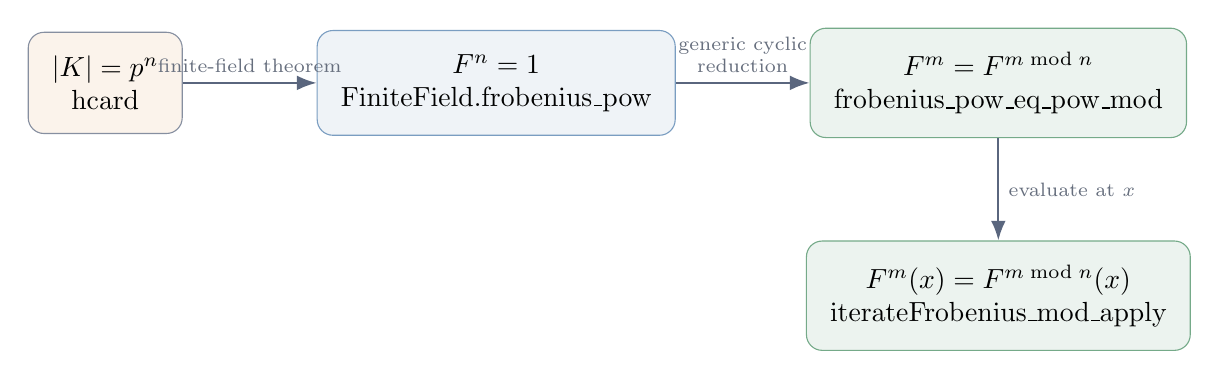
\begin{tikzpicture}[node distance=13mm and 17mm]
  \node[box,fill=orange!9] (card) {$|K|=p^n$\\\code{hcard}};
  \node[theorem,right=of card] (period) {$F^n=1$\\\code{FiniteField.frobenius\_pow}};
  \node[normal,right=of period] (mod) {$F^m=F^{m\bmod n}$\\\code{frobenius\_pow\_eq\_pow\_mod}};
  \node[normal,below=of mod] (point) {$F^m(x)=F^{m\bmod n}(x)$\\\code{iterateFrobenius\_mod\_apply}};
  \draw[flow] (card)--node[label,above]{finite-field theorem}(period);
  \draw[flow] (period)--node[label,above]{generic cyclic\\reduction}(mod);
  \draw[flow] (mod)--node[label,right]{evaluate at $x$}(point);
\end{tikzpicture}
\end{center}

\vspace{2mm}
\begin{minipage}[t]{.48\textwidth}
\decision{Recommended declarations}
\begin{leansmall}
theorem frobenius_pow_eq_pow_mod
    (hcard : Fintype.card K = p ^ n) (m : Nat) :
    frobenius K p ^ m =
      frobenius K p ^ (m % n) :=
  pow_eq_pow_mod m (FiniteField.frobenius_pow hcard)

 theorem iterateFrobenius_mod_apply
    (hcard : Fintype.card K = p ^ n)
    (m : Nat) (x : K) :
    iterateFrobenius K p m x =
      iterateFrobenius K p (m % n) x := by
  rw [iterateFrobenius_eq_pow,
      iterateFrobenius_eq_pow,
      frobenius_pow_eq_pow_mod hcard m]
\end{leansmall}
\end{minipage}\hfill
\begin{minipage}[t]{.48\textwidth}
\decision{The four API decisions}
\begin{center}
\renewcommand{\arraystretch}{1.35}
\begin{tabular}{>{\raggedright\arraybackslash}p{.40\linewidth}p{.49\linewidth}}
\toprule
Question & Decision\\ \midrule
Which orientation? & unrestricted exponent on the left\\
Global simplification? & no \code{[simp]} attribute\\
Where to place it? & after \code{FiniteField.frobenius\_pow}\\
Pointwise name? & \code{iterateFrobenius\_mod\_apply}\\
\bottomrule
\end{tabular}
\end{center}

\vspace{2mm}
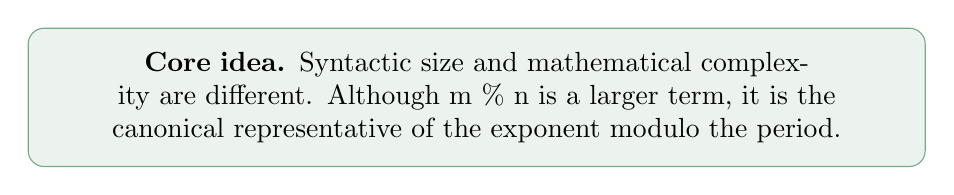
\begin{tikzpicture}
\node[normal,text width=.89\linewidth] {\textbf{Core idea.} Syntactic size and mathematical complexity are different. Although \code{m \% n} is a larger term, it is the canonical representative of the exponent modulo the period.};
\end{tikzpicture}
\end{minipage}

\vfill
\begin{center}\small\color{muted}Companion to \code{FROBENIUS\_API\_REVIEW.md} and the checked examples module.\end{center}
\newpage

% PAGE 2
\begin{center}
{\Large\bfseries\color{navy} 1. Why the ``larger'' right-hand side is the normal form}
\end{center}

Let $F=\operatorname{Frob}_p$.  Since $F^n=1$, the value of $F^m$ depends only on the residue class of $m$ modulo $n$.  Normalization chooses the canonical representative $m\bmod n$.

\begin{center}
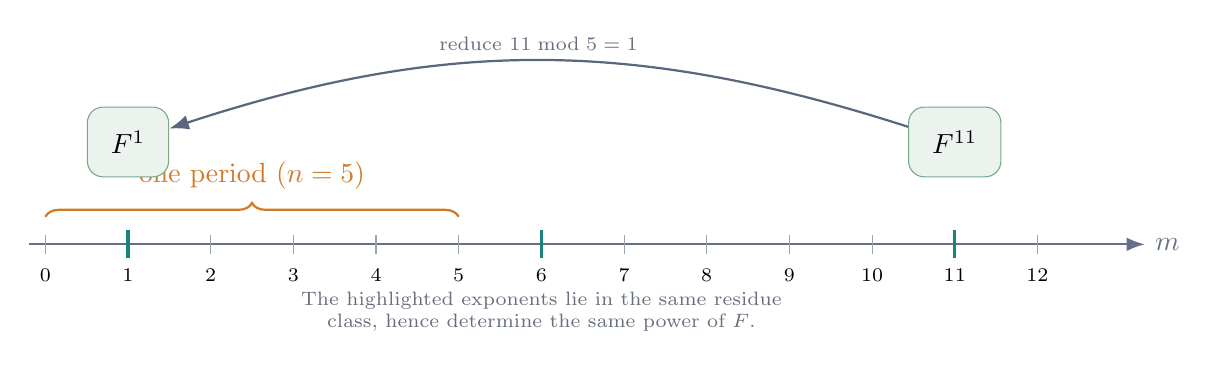
\begin{tikzpicture}[x=1.05cm,y=1cm]
  \draw[-{Latex},thick,navy!70] (-.2,0)--(13.3,0) node[right] {$m$};
  \foreach \x in {0,...,12} \draw[navy!45] (\x,.12)--(\x,-.12);
  \foreach \x/\lab in {0/0,1/1,2/2,3/3,4/4,5/5,6/6,7/7,8/8,9/9,10/10,11/11,12/12}
    \node[below=2pt,font=\scriptsize] at (\x,-.12) {\lab};
  \draw[decorate,decoration={brace,amplitude=5pt},orange,thick] (0,.35)--(5,.35)
    node[midway,above=6pt,text=orange] {one period ($n=5$)};
  \node[normal] (a) at (11,1.3) {$F^{11}$};
  \node[normal] (b) at (1,1.3) {$F^{1}$};
  \draw[flow,bend right=18] (a) to node[label,above]{reduce $11\bmod5=1$} (b);
  \foreach \x in {1,6,11} \draw[teal,very thick] (\x,.18)--(\x,-.18);
  \node[label,text width=8cm] at (6,-.85) {The highlighted exponents lie in the same residue class, hence determine the same power of $F$.};
\end{tikzpicture}
\end{center}

\begin{multicols}{2}
\decision{Three aligned precedents}

The recommended orientation is not an isolated style preference.  It follows the whole theorem chain:

\begin{center}
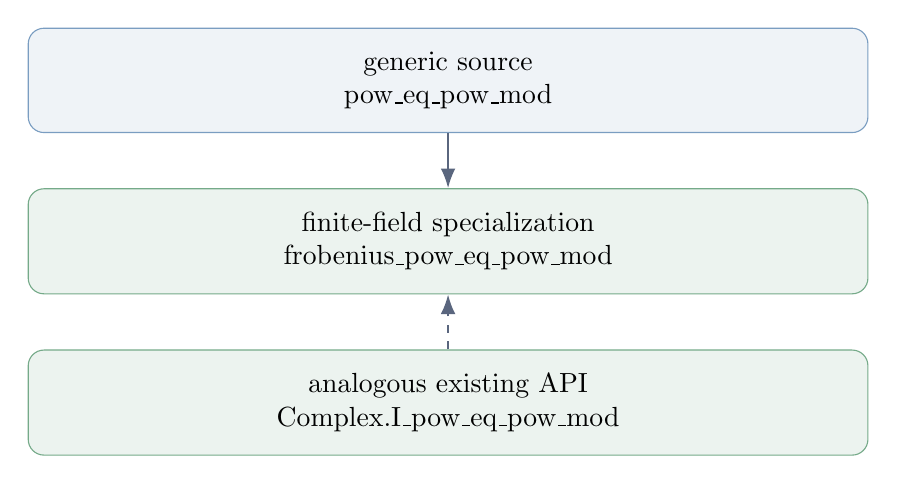
\begin{tikzpicture}[node distance=7mm]
\node[theorem,text width=.83\linewidth] (g) {generic source\\\code{pow\_eq\_pow\_mod}};
\node[normal,text width=.83\linewidth,below=of g] (f) {finite-field specialization\\\code{frobenius\_pow\_eq\_pow\_mod}};
\node[normal,text width=.83\linewidth,below=of f] (c) {analogous existing API\\\code{Complex.I\_pow\_eq\_pow\_mod}};
\draw[flow] (g)--(f);
\draw[flow,dashed] (c)--(f);
\end{tikzpicture}
\end{center}

All three read
\[
\text{arbitrary power}=\text{reduced power}.
\]
The wrapper therefore preserves the direction of its generic source theorem.

\columnbreak
\decision{Two notions of complexity}

\begin{center}
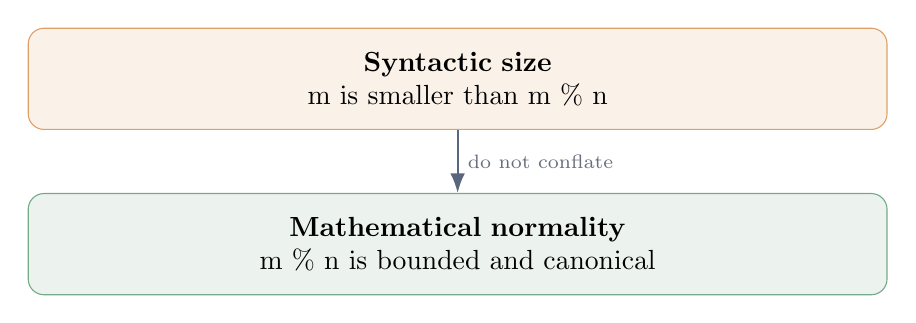
\begin{tikzpicture}[node distance=8mm]
\node[caution,text width=.85\linewidth] (syntax) {\textbf{Syntactic size}\\\code{m} is smaller than \code{m \% n}};
\node[normal,text width=.85\linewidth,below=of syntax] (math) {\textbf{Mathematical normality}\\\code{m \% n} is bounded and canonical};
\draw[flow] (syntax)--node[label,right]{do not conflate}(math);
\end{tikzpicture}
\end{center}

The goal of this theorem is periodic normalization, not raw AST-size reduction.  The right-hand side:
\begin{itemize}
\item records the period explicitly;
\item bounds the exponent by $n$ when $n>0$;
\item makes equivalent iterates visibly comparable;
\item exposes a canonical representative for later proofs.
\end{itemize}

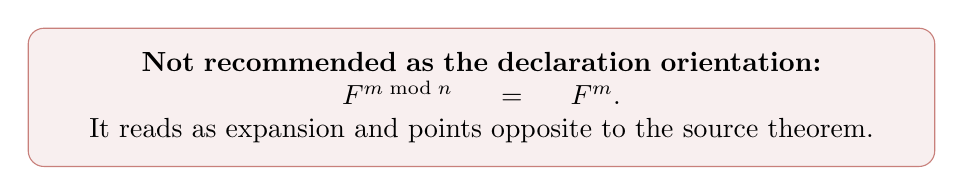
\begin{tikzpicture}
\node[bad,text width=.9\linewidth] {\textbf{Not recommended as the declaration orientation:}\\$F^{m\bmod n}=F^m$.\\It reads as expansion and points opposite to the source theorem.};
\end{tikzpicture}
\end{multicols}

\vfill
\begin{center}
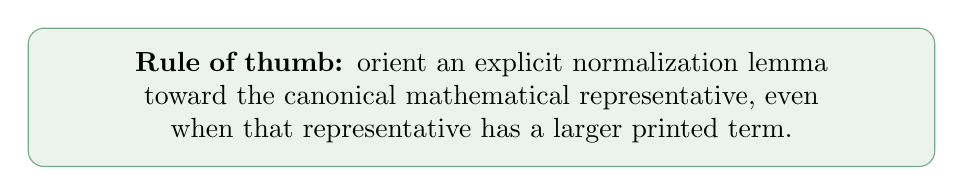
\begin{tikzpicture}
\node[normal,text width=.9\linewidth] {\textbf{Rule of thumb:} orient an explicit normalization lemma toward the canonical mathematical representative, even when that representative has a larger printed term.};
\end{tikzpicture}
\end{center}
\newpage

% PAGE 3
\begin{center}
{\Large\bfseries\color{navy} 2. Explicit rewrite, not global simplification}
\end{center}

The orientation answers ``what is the normal form?''  The \code{[simp]} decision answers a different question: ``should every simplifier invocation perform this normalization automatically?''

\begin{center}
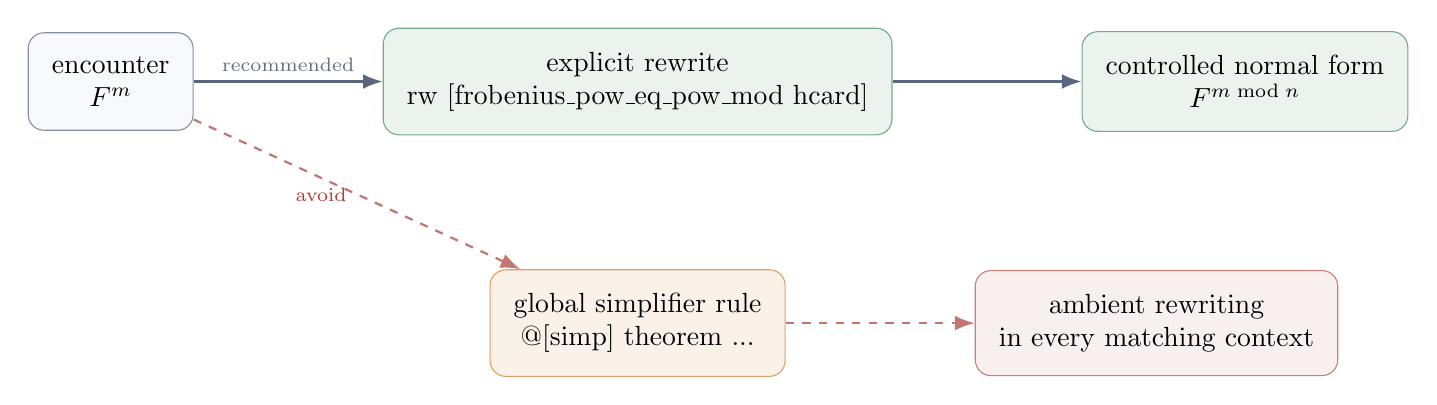
\begin{tikzpicture}[node distance=17mm and 24mm]
\node[box] (term) {encounter\\$F^m$};
\node[normal,right=of term] (explicit) {explicit rewrite\\\code{rw [frobenius\_pow\_eq\_pow\_mod hcard]}};
\node[caution,below=of explicit] (simp) {global simplifier rule\\\code{@[simp] theorem ...}};
\node[normal,right=of explicit] (controlled) {controlled normal form\\$F^{m\bmod n}$};
\node[bad,right=of simp] (ambient) {ambient rewriting\\in every matching context};
\draw[flow] (term)--node[label,above]{recommended}(explicit);
\draw[flow] (explicit)--(controlled);
\draw[flow,dashed,draw=red!70] (term)--node[label,left,text=red]{avoid}(simp);
\draw[flow,dashed,draw=red!70] (simp)--(ambient);
\end{tikzpicture}
\end{center}

\begin{multicols}{2}
\decision{Why explicit rewriting fits}
\begin{itemize}
\item The cardinality witness \code{hcard} is meaningful local data.
\item Users decide exactly where exponent reduction is useful.
\item Proof scripts advertise the normalization step.
\item The theorem remains available in either direction via \code{rw} or symmetry.
\item The term-size concern stays local rather than becoming simplifier policy.
\end{itemize}

\begin{lean}
-- Hom-level normalization
rw [FiniteField.frobenius_pow_eq_pow_mod hcard]

-- Pointwise normalization
rw [FiniteField.iterateFrobenius_mod_apply hcard]
\end{lean}

\columnbreak
\decision{Orientation does not forbid reverse use}

A theorem has a preferred reading direction, but equality remains symmetric.  Expand only at the call site that needs it:

\begin{lean}
exact
  (FiniteField.iterateFrobenius_mod_apply
    hcard m x).symm
\end{lean}

\begin{center}
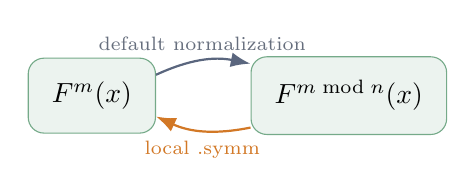
\begin{tikzpicture}[node distance=12mm]
\node[normal] (full) {$F^m(x)$};
\node[normal,right=of full] (reduced) {$F^{m\bmod n}(x)$};
\draw[flow] (full) to[bend left=18] node[label,above]{default normalization}(reduced);
\draw[flow,draw=orange] (reduced) to[bend left=18] node[label,below,text=orange]{local \code{.symm}}(full);
\end{tikzpicture}
\end{center}

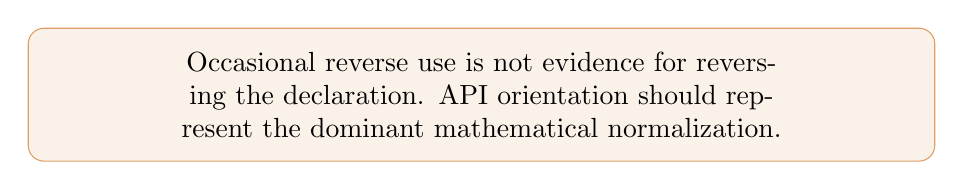
\begin{tikzpicture}
\node[caution,text width=.9\linewidth] {Occasional reverse use is not evidence for reversing the declaration.  API orientation should represent the dominant mathematical normalization.};
\end{tikzpicture}
\end{multicols}

\vspace{2mm}
\decision{Decision table}
\begin{center}
\renewcommand{\arraystretch}{1.35}
\begin{tabular}{p{.27\linewidth}p{.28\linewidth}p{.34\linewidth}}
\toprule
Situation & Tool & Why\\ \midrule
Normalize one hom expression & \code{rw [frobenius\_pow\_eq\_pow\_mod hcard]} & direct algebraic equality\\
Normalize one element expression & \code{rw [iterateFrobenius\_mod\_apply hcard]} & hides ring-hom powers\\
Need the unreduced form & theorem with \code{.symm}, or \code{rw [← ...]} & explicit, exceptional expansion\\
Routine unrelated simplification & leave these theorems unused & avoids global policy and term churn\\
\bottomrule
\end{tabular}
\end{center}
\newpage

% PAGE 4
\begin{center}
{\Large\bfseries\color{navy} 3. Two API layers for two kinds of clients}
\end{center}

The hom-level and pointwise statements express the same mathematics, but they serve different proof interfaces.

\begin{center}
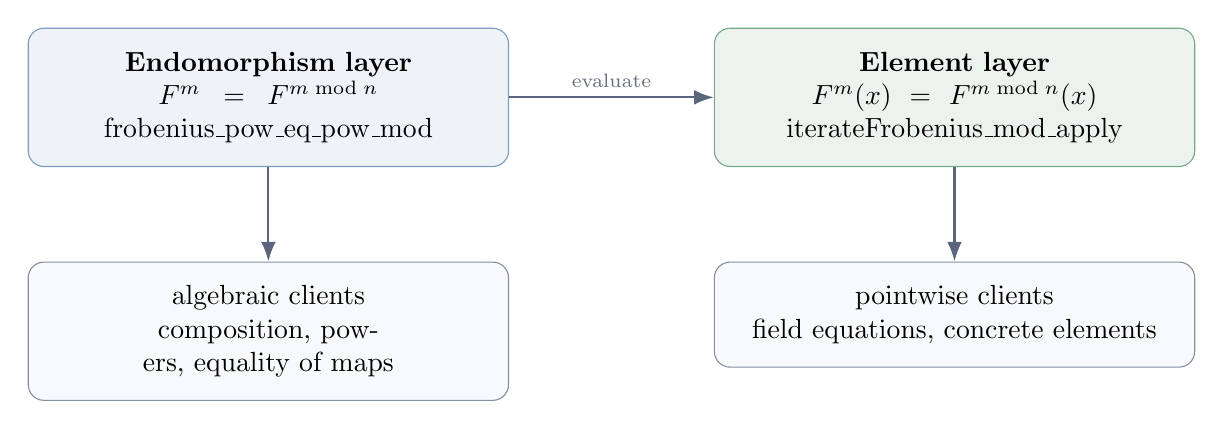
\begin{tikzpicture}[node distance=12mm and 26mm]
\node[theorem,text width=5.5cm] (hom) {\textbf{Endomorphism layer}\\$F^m=F^{m\bmod n}$\\\code{frobenius\_pow\_eq\_pow\_mod}};
\node[normal,text width=5.5cm,right=of hom] (pt) {\textbf{Element layer}\\$F^m(x)=F^{m\bmod n}(x)$\\\code{iterateFrobenius\_mod\_apply}};
\node[box,text width=5.5cm,below=of hom] (hc) {algebraic clients\\composition, powers, equality of maps};
\node[box,text width=5.5cm,below=of pt] (pc) {pointwise clients\\field equations, concrete elements};
\draw[flow] (hom)--(pt) node[label,midway,above]{evaluate};
\draw[flow] (hom)--(hc);
\draw[flow] (pt)--(pc);
\end{tikzpicture}
\end{center}

\begin{multicols}{2}
\decision{Hom-level example}
\begin{lean}
example (hcard : Fintype.card K = p ^ n)
    (m : Nat) :
    frobenius K p ^ (m + n) =
      frobenius K p ^ ((m + n) % n) := by
  rw [FiniteField.frobenius_pow_eq_pow_mod hcard]
\end{lean}

Use this form when the surrounding goal already treats Frobenius as a ring endomorphism.  It preserves the structural level and can be transported or composed as an equality of maps.

\decision{Minimal proof architecture}
\begin{center}

\begin{tikzpicture}[node distance=7mm]
\node[theorem,text width=.85\linewidth] (a) {\code{frobenius\_pow hcard}\\$F^n=1$};
\node[normal,text width=.85\linewidth,below=of a] (b) {\code{pow\_eq\_pow\_mod m}\\$F^m=F^{m\bmod n}$};
\draw[flow] (a)--(b);
\end{tikzpicture}
\end{center}
The first declaration is a direct generic specialization, so it belongs immediately beside its source theorem.

\columnbreak
\decision{Pointwise example}
\begin{lean}
example (hcard : Fintype.card K = p ^ n)
    (m : Nat) (x : K) :
    iterateFrobenius K p (m + n) x =
      iterateFrobenius K p ((m + n) % n) x := by
  rw [FiniteField.iterateFrobenius_mod_apply hcard]
\end{lean}

This wrapper keeps implementation details out of element-level proofs: clients need not manually expose \code{iterateFrobenius} as a power of a ring hom.

\decision{Why the name ends in \code{\_apply}}
\begin{center}
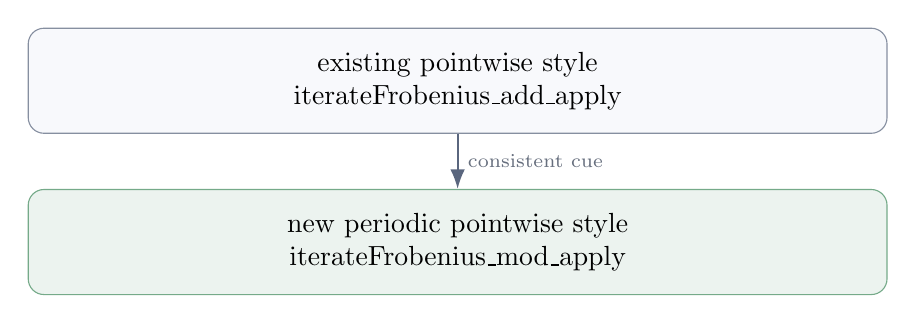
\begin{tikzpicture}[node distance=7mm]
\node[box,text width=.85\linewidth] (existing) {existing pointwise style\\\code{iterateFrobenius\_add\_apply}};
\node[normal,text width=.85\linewidth,below=of existing] (new) {new periodic pointwise style\\\code{iterateFrobenius\_mod\_apply}};
\draw[flow] (existing)--node[label,right]{consistent cue}(new);
\end{tikzpicture}
\end{center}
The suffix tells readers that the theorem concludes an equality after application to an element, distinguishing it at the call site from the ring-hom equality.
\end{multicols}

\vfill
\begin{center}
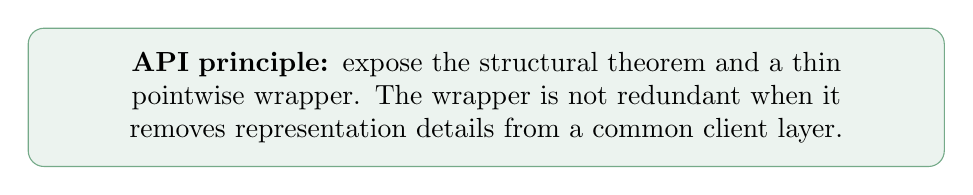
\begin{tikzpicture}
\node[normal,text width=.91\linewidth] {\textbf{API principle:} expose the structural theorem and a thin pointwise wrapper.  The wrapper is not redundant when it removes representation details from a common client layer.};
\end{tikzpicture}
\end{center}
\newpage

% PAGE 5
\begin{center}
{\Large\bfseries\color{navy} 4. Placement, edge cases, and review checklist}
\end{center}

\begin{multicols}{2}
\decision{Recommended source order}

\begin{center}
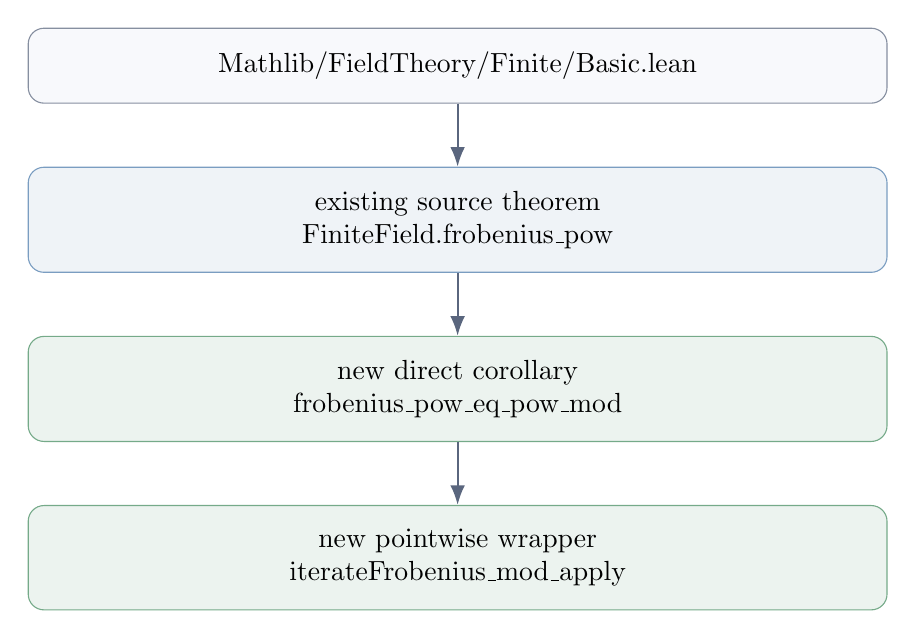
\begin{tikzpicture}[node distance=8mm]
\node[box,text width=.85\linewidth] (basic) {\code{Mathlib/FieldTheory/Finite/Basic.lean}};
\node[theorem,text width=.85\linewidth,below=of basic] (period) {existing source theorem\\\code{FiniteField.frobenius\_pow}};
\node[normal,text width=.85\linewidth,below=of period] (hom) {new direct corollary\\\code{frobenius\_pow\_eq\_pow\_mod}};
\node[normal,text width=.85\linewidth,below=of hom] (point) {new pointwise wrapper\\\code{iterateFrobenius\_mod\_apply}};
\draw[flow] (basic)--(period);
\draw[flow] (period)--(hom);
\draw[flow] (hom)--(point);
\end{tikzpicture}
\end{center}

This order keeps proof dependencies visible.  No additional finite-field machinery is required beyond the existing basic module.

\decision{The $n=0$ edge case}

No hypothesis \code{0 < n} is needed:
\[
m\bmod 0=m,
\]
so the conclusion becomes $F^m=F^m$.  Moreover, in the intended field setting the premise $|K|=p^0=1$ cannot describe a field's cardinality.  The statement is already total and correct without an artificial positivity side condition.

\columnbreak
\decision{What the final API says}

\begin{center}
\renewcommand{\arraystretch}{1.5}
\begin{tabular}{p{.51\linewidth}p{.28\linewidth}}
\toprule
Choice & Verdict\\ \midrule
Unrestricted exponent on left & \yes\\
Modulo exponent on right & \yes\\
Match generic theorem direction & \yes\\
Provide hom-level theorem & \yes\\
Provide pointwise wrapper & \yes\\
Use \code{\_apply} pointwise suffix & \yes\\
Place after \code{frobenius\_pow} & \yes\\
Add \code{0 < n} & \no\\
Mark either theorem \code{[simp]} & \no\\
Reverse declaration by default & \no\\
\bottomrule
\end{tabular}
\end{center}

\decision{Submission checklist}
\begin{itemize}
\item[$\square$] Preserve theorem orientation.
\item[$\square$] Keep both declarations free of \code{[simp]}.
\item[$\square$] Put the direct corollary beside \code{frobenius\_pow}.
\item[$\square$] Use the pointwise \code{\_mod\_apply} suffix.
\item[$\square$] Include endomorphism, pointwise, and reverse-use examples.
\item[$\square$] Build the target and inspect theorem axioms.
\end{itemize}
\end{multicols}

\vspace{3mm}
\begin{center}
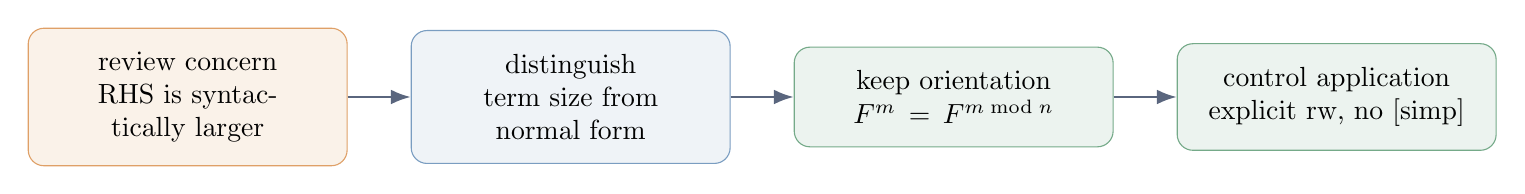
\begin{tikzpicture}[node distance=10mm and 8mm]
\node[caution,text width=3.45cm] (concern) {review concern\\RHS is syntactically larger};
\node[theorem,text width=3.45cm,right=of concern] (distinguish) {distinguish\\term size from normal form};
\node[normal,text width=3.45cm,right=of distinguish] (orient) {keep orientation\\$F^m=F^{m\bmod n}$};
\node[normal,text width=3.45cm,right=of orient] (policy) {control application\\explicit \code{rw}, no \code{[simp]}};
\draw[flow] (concern)--(distinguish);
\draw[flow] (distinguish)--(orient);
\draw[flow] (orient)--(policy);
\end{tikzpicture}
\end{center}

\vspace{5mm}
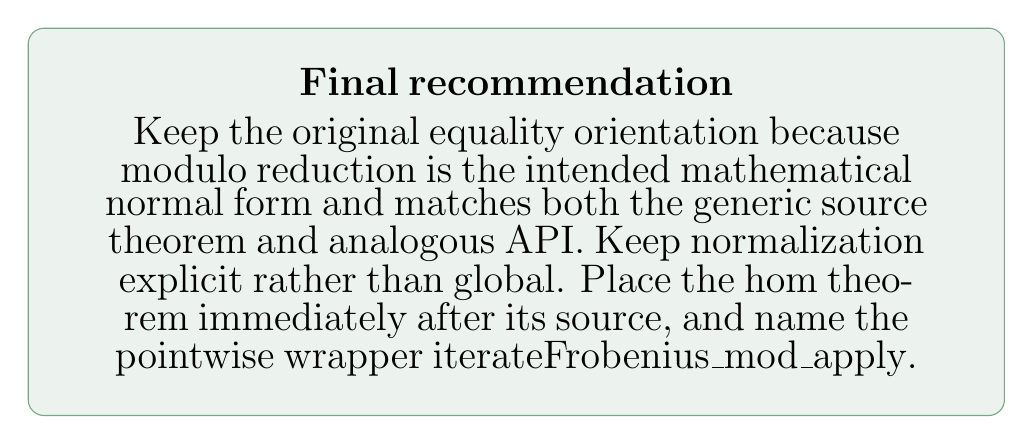
\begin{tikzpicture}
\node[normal,text width=.94\linewidth,inner sep=5mm] {\Large\textbf{Final recommendation}\\[2mm]
Keep the original equality orientation because modulo reduction is the intended mathematical normal form and matches both the generic source theorem and analogous API.  Keep normalization explicit rather than global.  Place the hom theorem immediately after its source, and name the pointwise wrapper \code{iterateFrobenius\_mod\_apply}.};
\end{tikzpicture}

\vfill
\begin{center}\small\color{muted}
The corresponding Lean declarations and all three usage modes are provided in\\
\code{MathlibExtras/FieldTheory/Finite/FrobeniusPeriod.lean} and\\
\code{MathlibExtras/FieldTheory/Finite/FrobeniusPeriodExamples.lean}.
\end{center}


\newpage
% PAGE 6
\begin{center}
{\Large\bfseries\color{navy} Appendix A. What the Lean and Mathlib sources actually do}
\end{center}

A regular-expression survey of Lean 4.28.0 and the checked-out Mathlib revision found a broad family of declarations that deliberately place a reduced residue expression on the right.  These are stronger precedents than the complex-number example alone.

\begin{center}
\renewcommand{\arraystretch}{1.32}
\begin{tabular}{p{.36\linewidth}p{.43\linewidth}p{.10\linewidth}}
\toprule
Declaration & Equality shape & \code{[simp]}?\\ \midrule
\code{pow\_eq\_pow\_mod} & $a^m=a^{m\bmod n}$ & no\\
\code{Complex.I\_pow\_eq\_pow\_mod} & $I^m=I^{m\bmod4}$ & no\\
\code{Int.units\_pow\_eq\_pow\_mod\_two} & $u^m=u^{m\bmod2}$ & no\\
\code{neg\_one\_pow\_eq\_pow\_mod\_two} & $(-1)^m=(-1)^{m\bmod2}$ & no\\
\code{χ₄\_nat\_mod\_four} & $\chi_4(m)=\chi_4(m\bmod4)$ & no\\
\code{χ₈\_nat\_mod\_eight} & $\chi_8(m)=\chi_8(m\bmod8)$ & no\\
\code{legendreSym.mod} & $(\frac ap)=(\frac{a\bmod p}{p})$ & no\\
\code{jacobiSym.mod\_left} & $J(a\mid b)=J(a\bmod b\mid b)$ & no\\
\code{jacobiSym.mod\_right} & $J(a\mid b)=J(a\mid b\bmod(4|a|))$ & no\\
\bottomrule
\end{tabular}
\end{center}

\begin{center}
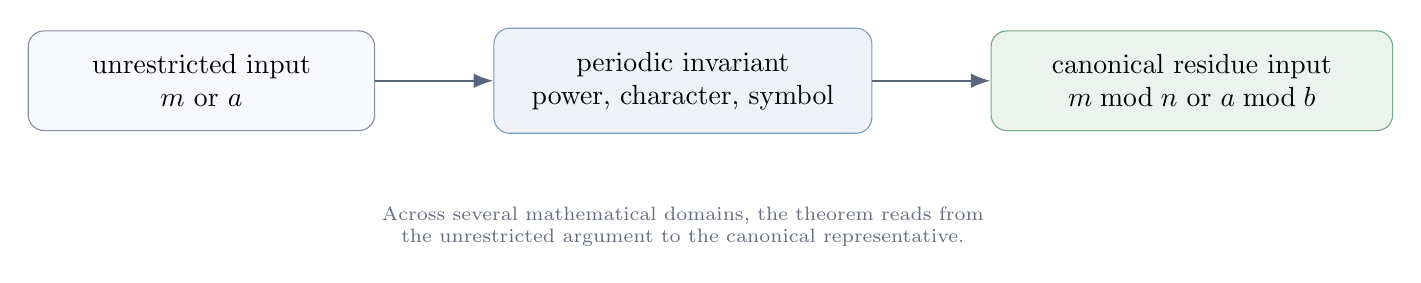
\begin{tikzpicture}[node distance=10mm and 15mm]
\node[box,text width=3.8cm] (input) {unrestricted input\\$m$ or $a$};
\node[theorem,text width=4.2cm,right=of input] (invariant) {periodic invariant\\power, character, symbol};
\node[normal,text width=4.5cm,right=of invariant] (residue) {canonical residue input\\$m\bmod n$ or $a\bmod b$};
\draw[flow] (input)--(invariant);
\draw[flow] (invariant)--(residue);
\node[label,text width=13cm,below=8mm of invariant] {Across several mathematical domains, the theorem reads from the unrestricted argument to the canonical representative.};
\end{tikzpicture}
\end{center}

\begin{multicols}{2}
\decision{Especially useful evidence}

The character and symbol declarations show that this convention is not peculiar to powers.  Their RHS may add casts, products inside a modulus, or \code{natAbs}; it is still preferred because it identifies the canonical residue data on which the invariant depends.

\begin{leansmall}
theorem χ₄_nat_mod_four (n : Nat) :
  χ₄ n = χ₄ (n % 4 : Nat)

protected theorem legendreSym.mod (a : Int) :
  legendreSym p a = legendreSym p (a % p)

 theorem jacobiSym.mod_right (a : Int) ... :
  J(a | b) = J(a | b % (4 * a.natAbs))
\end{leansmall}

\columnbreak
\decision{How the scan was performed}

Multiple broad regex families were used, then candidate declarations were inspected manually:
\begin{itemize}
\item multiline theorem statements with \code{mod} in the name and \code{\%} on an equality RHS;
\item periodicity families containing \code{pow\_eq\_pow\_mod}, \code{iterate\_mod}, \code{mod\_left}, or \code{mod\_right};
\item broad equalities whose RHS contains conditionals, compositions, maps, products, or arithmetic structure.
\end{itemize}

This is a source survey rather than a parser-based census.  Exact commands, revisions, file paths, and line references are recorded in \code{CODEBASE\_PATTERN\_SURVEY.md}.

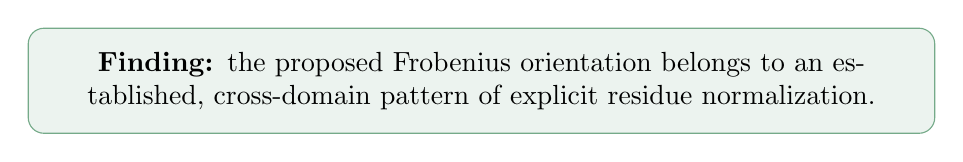
\begin{tikzpicture}
\node[normal,text width=.9\linewidth] {\textbf{Finding:} the proposed Frobenius orientation belongs to an established, cross-domain pattern of explicit residue normalization.};
\end{tikzpicture}
\end{multicols}

\newpage
% PAGE 7
\begin{center}
{\Large\bfseries\color{navy} Appendix B. Counter-patterns and larger RHSs}
\end{center}

A fair survey also finds the reverse direction.  The difference clarifies why \emph{simp policy}, not syntax-tree size alone, matters.

\begin{center}
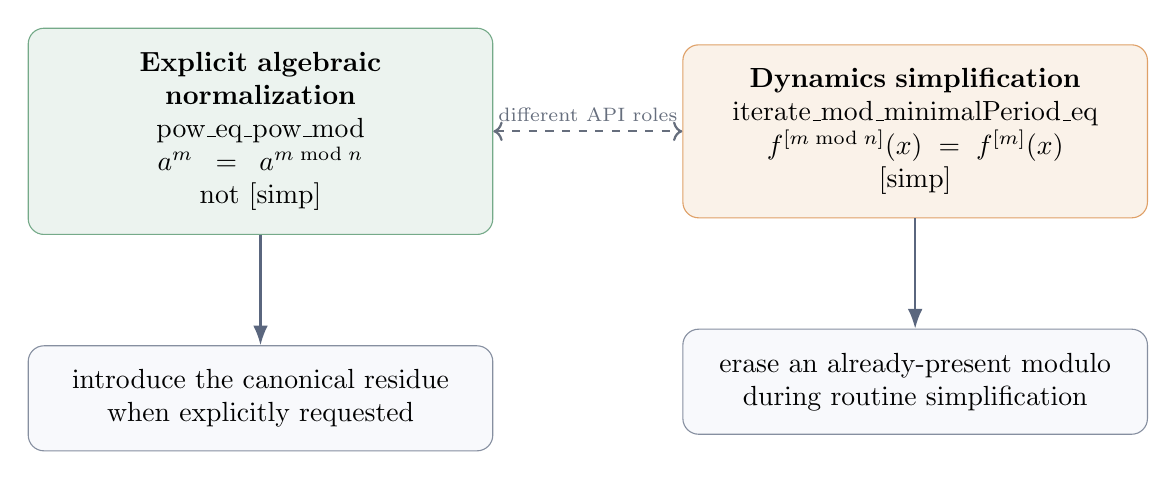
\begin{tikzpicture}[node distance=14mm and 24mm]
\node[normal,text width=5.3cm] (explicit) {\textbf{Explicit algebraic normalization}\\\code{pow\_eq\_pow\_mod}\\$a^m=a^{m\bmod n}$\\not \code{[simp]}};
\node[caution,text width=5.3cm,right=of explicit] (simp) {\textbf{Dynamics simplification}\\\code{iterate\_mod\_minimalPeriod\_eq}\\$f^{[m\bmod n]}(x)=f^{[m]}(x)$\\\code{[simp]}};
\node[box,text width=5.3cm,below=of explicit] (goal1) {introduce the canonical residue\\when explicitly requested};
\node[box,text width=5.3cm,below=of simp] (goal2) {erase an already-present modulo\\during routine simplification};
\draw[flow] (explicit)--(goal1);
\draw[flow] (simp)--(goal2);
\draw[<->,thick,dashed,draw=muted] (explicit)--node[label,above]{different API roles}(simp);
\end{tikzpicture}
\end{center}

\begin{multicols}{2}
\decision{The reverse-oriented family}
\begin{leansmall}
theorem IsPeriodicPt.iterate_mod_apply ... :
  f^[m % n] x = f^[m] x

@[simp] theorem iterate_mod_minimalPeriod_eq :
  f^[n % minimalPeriod f x] x = f^[n] x

@[simp] theorem pow_mod_period_smul ... :
  m ^ (n % period m a) • a = m ^ n • a
\end{leansmall}

This does not undermine the recommendation.  It demonstrates that declarations optimized for simplification can choose a different normal form from explicit normalization wrappers.  The Frobenius theorem is a direct specialization of the non-\code{[simp]} group-theoretic theorem.

\decision{Interpretation}
\begin{center}
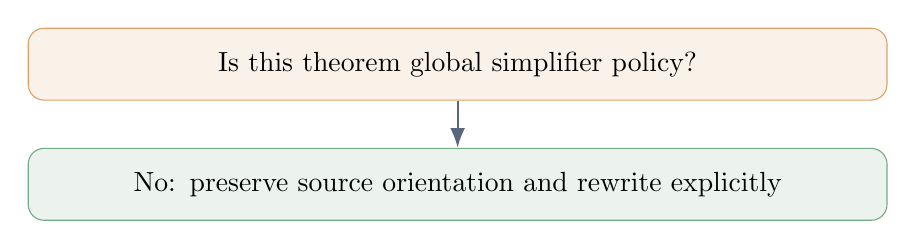
\begin{tikzpicture}[node distance=6mm]
\node[caution,text width=.85\linewidth] (q) {Is this theorem global simplifier policy?};
\node[normal,text width=.85\linewidth,below=of q] (a) {No: preserve source orientation and rewrite explicitly};
\draw[flow] (q)--(a);
\end{tikzpicture}
\end{center}

\columnbreak
\decision{Larger RHSs beyond modulo}

Lean core and Mathlib routinely expose a larger but more informative RHS:
\begin{leansmall}
-- Core arithmetic
Int.add_emod:
  (a + b) % n = (a % n + b % n) % n

Int.fmod_eq_emod:
  fmod a b = a % b +
    if 0 ≤ b ∨ b ∣ a then 0 else b

-- Core computation
Thunk.sizeOf_eq:
  sizeOf a = 1 + sizeOf a.get

-- Mathlib pointwise computation
CStarMatrix.one_apply:
  (1 : CStarMatrix n n A) i j =
    if i = j then 1 else 0

-- Mathlib structural exposure
Embedding.coe_trans:
  ⇑(f.trans g) = ⇑g ∘ ⇑f
\end{leansmall}

These are not direct Frobenius precedents, but they establish the broader design rule: orientation can expose canonical computational, pointwise, or compositional structure even when the printed RHS grows.
\end{multicols}

\vspace{3mm}
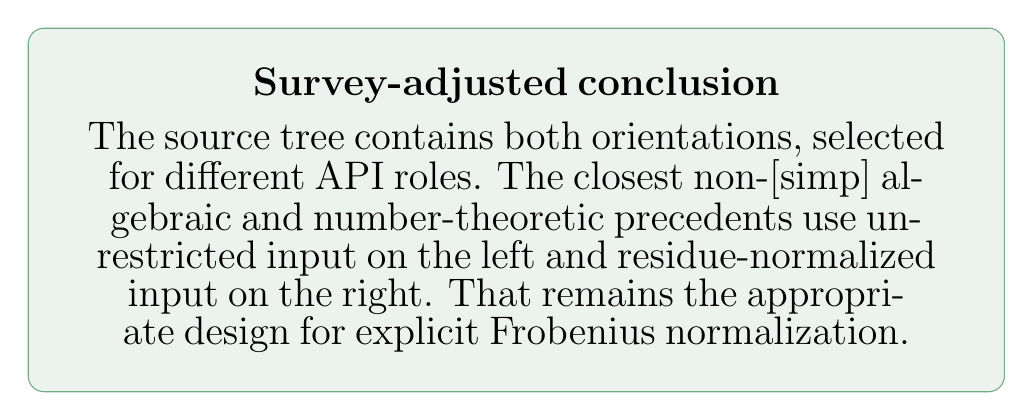
\begin{tikzpicture}
\node[normal,text width=.94\linewidth,inner sep=5mm] {\Large\textbf{Survey-adjusted conclusion}\\[2mm]
The source tree contains both orientations, selected for different API roles.  The closest non-\code{[simp]} algebraic and number-theoretic precedents use unrestricted input on the left and residue-normalized input on the right.  That remains the appropriate design for explicit Frobenius normalization.};
\end{tikzpicture}

\end{document}
